%%
%% This is file `sample-sigplan.tex',
%% generated with the docstrip utility.
%%
%% The original source files were:
%%
%% samples.dtx  (with options: `sigplan')
%% 
%% IMPORTANT NOTICE:
%% 
%% For the copyright see the source file.
%% 
%% Any modified versions of this file must be renamed
%% with new filenames distinct from sample-sigplan.tex.
%% 
%% For distribution of the original source see the terms
%% for copying and modification in the file samples.dtx.
%% 
%% This generated file may be distributed as long as the
%% original source files, as listed above, are part of the
%% same distribution. (The sources need not necessarily be
%% in the same archive or directory.)
%%
%%
%% Commands for TeXCount
%TC:macro \cite [option:text,text]
%TC:macro \citep [option:text,text]
%TC:macro \citet [option:text,text]
%TC:envir table 0 1
%TC:envir table* 0 1
%TC:envir tabular [ignore] word
%TC:envir displaymath 0 word
%TC:envir math 0 word
%TC:envir comment 0 0
%%
%%
%% The first command in your LaTeX source must be the \documentclass
%% command.
%%
%% For submission and review of your manuscript please change the
%% command to \documentclass[manuscript, screen, review]{acmart}.
%%
%% When submitting camera ready or to TAPS, please change the command
%% to \documentclass[sigconf]{acmart} or whichever template is required
%% for your publication.
%%
%%
\documentclass[nonacm, sigplan]{acmart}

\usepackage{url}
\usepackage[ruled,noend,linesnumbered]{algorithm2e}
\usepackage{graphicx,color,psfrag}
\usepackage{amsmath}
\usepackage{amsfonts}
\usepackage{amssymb}
\usepackage{bigdelim}
\usepackage{dsfont}
\usepackage{color, soul}
\usepackage{graphicx}
\usepackage{caption}
\usepackage{subcaption}

%%
%% \BibTeX command to typeset BibTeX logo in the docs
\AtBeginDocument{%
  \providecommand\BibTeX{{%
    Bib\TeX}}}

%% Rights management information.  This information is sent to you
%% when you complete the rights form.  These commands have SAMPLE
%% values in them; it is your responsibility as an author to replace
%% the commands and values with those provided to you when you
%% complete the rights form.
\setcopyright{acmcopyright}
\copyrightyear{2018}
\acmYear{2018}
\acmDOI{XXXXXXX.XXXXXXX}

%% These commands are for a PROCEEDINGS abstract or paper.
\acmConference[Conference acronym 'XX]{Make sure to enter the correct
  conference title from your rights confirmation emai}{June 03--05,
  2018}{Woodstock, NY}
%%
%%  Uncomment \acmBooktitle if the title of the proceedings is different
%%  from ``Proceedings of ...''!
%%
%%\acmBooktitle{Woodstock '18: ACM Symposium on Neural Gaze Detection,
%%  June 03--05, 2018, Woodstock, NY}
\acmPrice{15.00}
\acmISBN{978-1-4503-XXXX-X/18/06}


%%
%% Submission ID.
%% Use this when submitting an article to a sponsored event. You'll
%% receive a unique submission ID from the organizers
%% of the event, and this ID should be used as the parameter to this command.
%%\acmSubmissionID{123-A56-BU3}

%%
%% For managing citations, it is recommended to use bibliography
%% files in BibTeX format.
%%
%% You can then either use BibTeX with the ACM-Reference-Format style,
%% or BibLaTeX with the acmnumeric or acmauthoryear sytles, that include
%% support for advanced citation of software artefact from the
%% biblatex-software package, also separately available on CTAN.
%%
%% Look at the sample-*-biblatex.tex files for templates showcasing
%% the biblatex styles.
%%

%%
%% The majority of ACM publications use numbered citations and
%% references.  The command \citestyle{authoryear} switches to the
%% "author year" style.
%%
%% If you are preparing content for an event
%% sponsored by ACM SIGGRAPH, you must use the "author year" style of
%% citations and references.
%% Uncommenting
%% the next command will enable that style.
%%\citestyle{acmauthoryear}


%%
%% end of the preamble, start of the body of the document source.
\begin{document}

%%
%% The "title" command has an optional parameter,
%% allowing the author to define a "short title" to be used in page headers.
\title[ICIIT 2024]{Grasp Generation with Depth Estimation from Color Images}

%%
%% The "author" command and its associated commands are used to define
%% the authors and their affiliations.
%% Of note is the shared affiliation of the first two authors, and the
%% "authornote" and "authornotemark" commands
%% used to denote shared contribution to the research.

\author{Van-Thiep Nguyen}
\affiliation{%
\institution{FPT University}
\city{Hanoi}
\country{Vietnam}
}
\email{thiepnvhe173027@fpt.edu.vn}

\author{Van-Duc Vu}
\affiliation{%
\institution{FPT University}
\city{Hanoi}
\country{Vietnam}
}
\email{ducvvhe176438@fpt.edu.vn}

\author{Ngoc-Anh Hoang}
\affiliation{%
\institution{FPT University}
\city{Hanoi}
\country{Vietnam}
}
\email{anhhnhe186401@fpt.edu.vn}

\author{Thu-Uyen Nguyen}
\affiliation{%
\institution{FPT University}
\city{Hanoi}
\country{Vietnam}
}
\email{uyennthe176614@fpt.edu.vn}

\author{Duy-Quang Vu}
\affiliation{%
\institution{FPT University}
\city{Hanoi}
\country{Vietnam}
}
\email{quangvdhe163133@fpt.edu.vn}

\author{Duc-Thanh Tran}
\affiliation{%
\institution{FPT University}
\city{Hanoi}
\country{Vietnam}
}
\email{thanhtdhe176812@fpt.edu.vn}

\author{Khanh-Toan Phan}
\affiliation{%
\institution{FPT University}
\city{Hanoi}
\country{Vietnam}
}
\email{toanpkhe170983@fpt.edu.vn}

\author{Anh-Truong Mai}
\affiliation{%
\institution{FPT University}
\city{Hanoi}
\country{Vietnam}
}
\email{TruongMAHE182474@fpt.edu.vn}

\author{Van-Hiep Duong}
\affiliation{%
\institution{FPT University}
\city{Hanoi}
\country{Vietnam}
}
\email{hiepdvhe181185@fpt.edu.vn}

\author{Cong-Trinh Tran}
\affiliation{%
\institution{FPT University}
\city{Hanoi}
\country{Vietnam}
}
\email{trinhtche160916@fpt.edu.vn}

\author{Ngoc-Trung Ho}
\affiliation{%
\institution{FPT University}
\city{Hanoi}
\country{Vietnam}
}
\email{trunghnhe172033@fpt.edu.vn}

\author{Quang-Tri Duong}
\affiliation{%
\institution{FPT University}
\city{Hanoi}
\country{Vietnam}
}
\email{TriDQGCH210221@fpt.edu.vn}

\author{Phuc-Quan Ngo}
\affiliation{%
\institution{FPT University}
\city{Hanoi}
\country{Vietnam}
}
\email{QuanNPGCH211110@fpt.edu.vn}

\author{Dinh-Cuong Hoang}
\affiliation{%
\institution{FPT University}
\city{Hanoi}
\country{Vietnam}
}
\email{cuonghd12@fe.edu.vn}

%%
%% By default, the full list of authors will be used in the page
%% headers. Often, this list is too long, and will overlap
%% other information printed in the page headers. This command allows
%% the author to define a more concise list
%% of authors' names for this purpose.
\renewcommand{\shortauthors}{V.T Nguyen et al.}

%%
%% The abstract is a short summary of the work to be presented in the
%% article.
\begin{abstract}
Grasp generation plays a fundamental role in robot manipulation, often relying on three-dimensional (3D) point cloud data acquired through specialized depth cameras. However, the limited availability of such sensors in practical scenarios emphasizes the necessity for alternative approaches. This paper introduces an innovative method for grasp generation directly from color (RGB) images, negating the reliance on dedicated depth sensors. The proposed method employs tailored deep learning techniques for depth estimation from color images. Instead of traditional depth sensors, our approach computes predicted point clouds from estimated depth images directly generated from RGB inputs. A significant contribution lies in the design of a fusion module adept at seamlessly integrating features extracted from RGB images with those inferred from the predicted point clouds. This fusion process significantly strengthens the grasp generation pipeline by strengthening the advantages of both modalities, yielding notably improved grasp configurations. Experimental evaluations on standard datasets validate the efficacy of our approach, demonstrating its superior performance in generating grasp configurations compared to existing methods.
\end{abstract}

%%
%% The code below is generated by the tool at http://dl.acm.org/ccs.cfm.
%% Please copy and paste the code instead of the example below.
%%
\begin{CCSXML}
<ccs2012>
   <concept>
       <concept_id>10010147.10010178.10010224</concept_id>
       <concept_desc>Computing methodologies~Computer vision</concept_desc>
       <concept_significance>500</concept_significance>
       </concept>
 </ccs2012>
\end{CCSXML}

\ccsdesc[500]{Computing methodologies~Computer vision}


%%
%% Keywords. The author(s) should pick words that accurately describe
%% the work being presented. Separate the keywords with commas.
\keywords{Pose estimation, robot vision systems , intelligent systems,   deep learning, supervised learning, machine vision.}
%% A "teaser" image appears between the author and affiliation
%% information and the body of the document, and typically spans the
%% page.

%\received{20 February 2007}
%\received[revised]{12 March 2009}
%\received[accepted]{5 June 2009}

%%
%% This command processes the author and affiliation and title
%% information and builds the first part of the formatted document.
\maketitle

\section{Introduction}
\label{sec:intro}

Grasp configuration generation stands as a critical element in robotic manipulation, and vision-based methodologies have played a pivotal role in addressing this challenge \cite{hoang2023grasp, hoang2022context, fang2020graspnet}. While model-based grasp generation has been prevalent, its limitations become apparent, particularly when confronting unknown objects \cite{du2021vision, hoang2020panoptic, hoang2020object, hoang2019object, hoang2016sub, hoang2022voting, vu2024occlusion, palleschi2020fully, chen2016innovative}. An alternative avenue involves generating grasp configurations directly from sensor data without presuming knowledge of the object's 3D model or pre-computed grasps, referred to as grasp generation or grasp detection \cite{fang2020graspnet, hoang2022context}. Current methods fall into two categories: planar grasping and six Degrees of Freedom (6-DoF) grasping. Planar grasping utilizes a simple yet effective representation defining grasps as oriented bounding boxes. While this low degree of freedom (DoF) representation simplifies the task to a detection problem, it restricts performance in 3D manipulation tasks. On the other hand, 6-DoF grasping offers greater dexterity, suitable for complex scenarios. However, accurate generation of 6-DoF grasps necessitates geometric information, leading many existing methods to rely on 3D point cloud data. Despite significant progress achieved by grasp generation methods using point clouds, challenges persist due to measurement noise, occlusions, and environmental interference, making generating feasible and reliable grasps in cluttered scenes difficult. Additionally, many methods require time-consuming multi-stage processing for sampling grasp candidates and evaluating grasp quality, while the unavailability of 3D point cloud data in numerous applications exacerbates this issue \cite{ten2017grasp, liang2019pointnetgpd, du2021vision}. In contrast to 3D point clouds, acquiring color (RGB) images is more cost-effective and straightforward. With the advancements in deep learning, tasks such as object detection or 6D object pose estimation from RGB images have exhibited remarkable performance. However, the domain of grasp detection from RGB images remains largely unexplored.

In this work, we present a deep learning approach for grasp generation, focusing exclusively on leveraging RGB images to achieve accurate grasp estimation, building upon our previous research efforts \cite{hoang2023grasp, hoang2022context}. To obtain crucial geometric information for prediction, we employ recent advancements in monocular depth estimation to extract 3D points. Using an RGB image and the predicted 3D point cloud, we introduce an adaptive fusion module to extract discriminative features. These features are then input into a deep Hough voting module, inspired by our prior works \cite{hoang2023grasp, hoang2022context}, which has demonstrated the effectiveness of voting mechanisms in addressing occlusions and ensuring collision-free grasps. Following the voting module, the collected votes undergo clustering and regression processes to precisely determine the essential grasp parameters. We evaluate the proposed method on a standard dataset and in a real-world robot grasping application. The results demonstrate promising outcomes, indicating that even with the utilization of only RGB images and estimated depth maps, we achieve noteworthy results. 
%
\section{Literature Review}
\label{sec:relatedwork}

\subsection{Learning-based Grasp Generation}

The grasp pose detection problem involves predicting multiple poses within a scene, enabling robots to manipulate objects effectively. Earlier approaches \cite{bicchi2000robotic, miller2003automatic} assumed complete 2D or 3D object knowledge or simplified objects as primitive shapes, facing limitations in obtaining accurate 3D models. Learning-based methods emerged, utilizing large-scale data and automated feature extraction. Some focused on 4-DoF grasp poses on the camera plane, known as "top-down grasping," restricting degrees of freedom and potentially missing crucial grasp poses, like those along object edges. In contrast, 6-DoF grasp poses offer increased flexibility and complexity, allowing grasping from various directions, necessitating six parameters to define location and rotation, with potential inclusion of additional degrees of freedom, like gripper width or height. Learning-based grasp generation can be categorized into two primary algorithmic methodologies for grasp synthesis: grasp pose sampling and and regressing grasp pose directly. Sampling-based approaches, like GPD \cite{ten2017grasp} and PointNetGPD \cite{liang2019pointnetgpd}, evaluate individual grasp samples. Despite dense sampling, they struggle in regions like the rims of objects where surface normals estimation is unreliable. Some methods, such as Lou et al. \cite{lou2020learning}, sample wrist angles independently, while others, like Kokic et al. \cite{kokic2020learning}, sample grasp, roll angles, and offset distances. However, these approaches often trade computation time for generated grasp poses, resulting in limited poses per scene and a focus on local object features. Direct regression methods, exemplified by Schmidt et al. \cite{schmidt2018grasping} and Yang et al. \cite{yang2021robotic}, predict grasp poses or transformation matrices directly from visual data, processing information holistically. Yet, approaches like GraspNet \cite{fang2020graspnet} and PointNet++ \cite{ni2020pointnet++}, utilizing entire scene point clouds, lack consideration for inter-object relationships, limiting performance in cluttered scenes and under occlusion. To overcome these limitations, our previous work \cite{hoang2023grasp, hoang2022context} leverage a voting mechanism and contextual information to directly generate grasp configurations from 3D point clouds, addressing challenges in occlusion common in manipulationThe proposed method aligns closely with our prior studies \cite{hoang2023grasp, hoang2022context}. However, rather than relying on 3D data from depth sensors, we explore the utilization of depth images estimated via a monocular depth estimation framework. 

\subsection{Monocular Depth Estimation}

The inception of monocular depth estimation was pioneered by \cite{saxena2005learning, saxena2008make3d}, employing hand-engineered features and Markov Random Fields (MRF). Subsequently, the advent of deep learning, spearheaded by Eigen et al. \cite{eigen2014depth}, revolutionized depth estimation. However, learned depth regression encounters challenges in the decoder phase due to the loss of fine details from successive convolution layers in neural networks. Numerous approaches have addressed this issue diversely. \cite{eigen2015predicting} introduced multi-scale networks to predict depth at multiple resolutions. Laina et al. \cite{laina2016deeper} enhanced a ResNet architecture with improved up-sampling blocks to mitigate information loss. Xu et al. \cite{xu2017multi} combined deep learning with conditional random fields (CRF) for feature fusion at different scales. Another line of research pursued multitask learning, simultaneously predicting semantic labels \cite{jiao2018look}, depth edges, and normals \cite{ramamonjisoa2019sharpnet, zhang2019pattern, lee2019big} to refine depth predictions. Kendall et al. \cite{kendall2018multi} explored uncertainty estimation's impact on scene understanding, while Yin et al. \cite{yin2019enforcing} used surface geometry to estimate 3D point clouds from predicted depth maps. Recent works by Bhat et al. propose a classification-based formulation for distance prediction [29]. Tian et al. \cite{chen2020improving} integrated attention blocks into the decoder, while Transformer-based architectures gained traction \cite{ranftl2021vision, yang2021transformer}.
%
\section{Materials and Methods}
\label{sec:methodology}

An overview of the proposed method is presented in Fig. \ref{fig:Overview}. Our approach consists of several key components, including depth estimation, attention-based adaptive fusion incorporating visual-guided 3D geometric feature and geometric-guided visual feature Learning, and voting-based grasp generation. These components work synergistically to enhance the dis- criminability and robustness of features, ultimately leading to more accurate and efficient grasp pose generation. We provide a detailed explanation of each of these components and their role in our system’s success.

%%%%%%%%%%%%%%%%%%%%%%%%%%%%%%%%%%%%%%%%%%%%%%%

\begin{figure*}[h!]
	\centering
	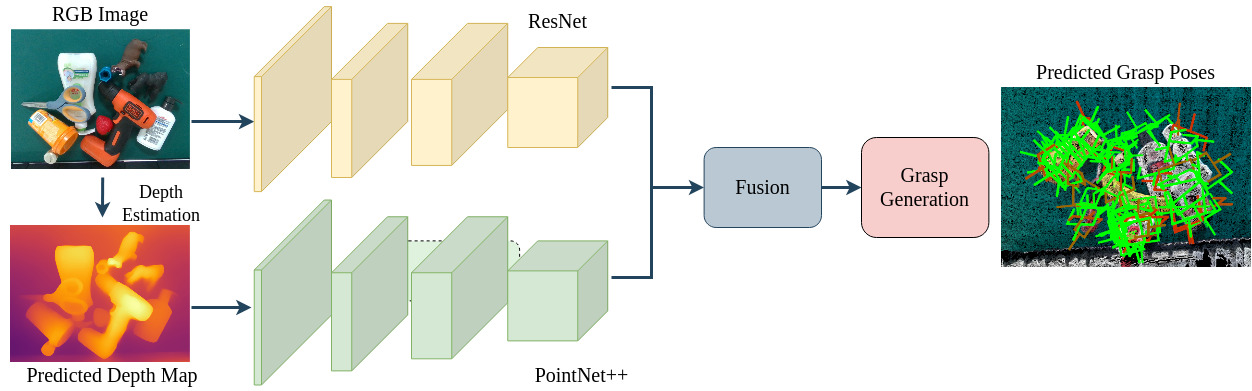
\includegraphics[width=0.98\linewidth]{figs/overview}
	\caption{Overview of our network architecture.}
	\label{fig:Overview}
\end{figure*}
%%%%%%%%%%%%%%%%%%%%%%%%%%%%%%%%%%%%%%%%%%%%%%

\subsection{Depth Estimation}

Existing monocular depth estimation methods are primarily tailored for large outdoor scenes, posing challenges when applied to relatively smaller objects intended for manipulation. To address this limitation, our focus is on enhancing the depth map quality specifically for such objects. We leverage two distinct depth estimation networks, DPT \cite{ranftl2021vision} and iDisc \cite{piccinelli2023idisc}, to derive individual depth images denoted as $\mathbf{I}_{d1}$ and $\mathbf{I}_{d2}$, respectively. By computing the disparity between these images, regions with significant differences beyond a predefined threshold are identified as uncertain areas. Our approach involves excluding these uncertain regions from the depth images and replacing the depth values within other areas with their mean values. This process aims to refine depth information specifically for small object manipulation, culminating in an enhanced and more accurate depth image, denoted as $\mathbf{I}_{d}$.

\subsection{Attention-based Adaptive Fusion Network}

Given a RGB image $\mathbf{I_v}$ and an estimated depth map $\mathbf{I_d}$, our initial step involves elevating the depth image $\mathbf{I_d}$ to a point cloud $\mathbf{P}$ using the camera intrinsic matrix. Subsequently, we employ ResNet34 \cite{he2016deep} and PointNet++ \cite{qi2017pointnet++} to extract visual features $\mathcal{F}_{vis}$ from RGB image and geometric feature $\mathcal{F}_{geo}$ from the point cloud $\mathbf{P}$ respectively. These networks facilitate bidirectional information flow through Visual-Guided Geometric Feature Learning (VGG) and Geometric-Guided Visual Feature Learning (GGV) modules, enabling each branch to utilize mutual local and global information for enhanced representation learning. \\

\textbf{Visual-Guided 3D Geometric Feature Learning}

To integrate visual information from $\mathcal{F}_{vis}^{i}$ into geometric features $\mathcal{F}_{geo}^{i}$ in the $i$-th stage, we introduce a novel Visual-Guided Geometric Feature Learning (VGG) module. Rather than globally compressing the RGB feature map and potentially losing intricate details, we utilize the aligned RGBD image. Each pixel's depth contributes to deriving its corresponding 3D point, establishing an XYZ map aligned with the RGB map. For every geometric feature paired with its 3D point coordinate, we retrieve visual features from $\mathcal{F}_{vis}$ by projecting its neighborhood, with a radius $r_1$, onto the image. Subsequently, we sample the $k_1$ nearest neighbor pixels within this region, gathering their visual features. In cases where fewer than $k_1$ pixels exist in the corresponding region, null features are padded. These collected visual features are integrated using max pooling and processed through Multi-Layer Perceptrons (MLPs) to match their channel size with the point cloud feature. This stage produces modified visual features $\mathcal{F}_{vis}^{'}$. Subsequently, we concatenate the integrated visual features $\mathcal{F}_{vis}^{'}$ with the geometric features $\mathcal{F}_{geo}^{i}$ and apply a shared MLP to obtain the fused geometric feature $\mathcal{F}_{geo}^{fus}$. Consequently, the network enriches $N$ 3D points with high-dimensional features, denoted as $\mathcal{P} = \lbrace p_i \rbrace_{i=1}^{N}$ and $\mathcal{F}_{geo}^{'} = \lbrace f_i \rbrace_{i=1}^{N}$, where $p_i = [ x_i; f_i ]$. Here, $x_i \in \mathbb{R}^{3}$ signifies the point's location in 3D space, and $f_i$ represents the associated feature vector. The enriched points $\lbrace p_{i} \rbrace_{i=1}^{N}$, now imbued with the fused features, are then inputted into our self-attention module to enhance the features $\mathcal{F}_{geo}^{ei}$. In accordance with \cite{zhao2021point, vaswani2017attention}, the self-attention module is defined as follows:


%%%%%%%%%%%%%%%%%%%%%
\begin{equation}
y_{i} = \sum_{p_{j} \in \mathcal{P}(i)} (\alpha(\gamma(p_{i},p_{j}) + \delta) \odot \beta(p_{j}))
\end{equation}
%%%%%%%%%%%%%%%%%%%%%

\noindent $\mathcal{P}(i) \subseteq \mathcal{P}$ refers to a set of points in the local neighborhood of $p_{i}$. $\alpha, \gamma, \delta$, and $\beta$ signify a mapping function, a relation function, a position encoding function, and pointwise feature transformation, respectively. The relation function $\gamma$ uses subtraction to output a vector representing the features of $p_i$ and $p_j$:

%%%%%%%%%%%%%%%%%%%%%
\begin{equation}
\gamma(p_{i},p_{j}) = \varphi(p_i) - \psi(p_j) 
\end{equation}
%%%%%%%%%%%%%%%%%%%%

\noindent Here, $\varphi$ and $\psi$ represent trainable transformations using multilayer perceptrons (MLPs). The mapping function $\alpha$ is an MLP with two linear layers and one ReLU nonlinearity, allowing the module to compute attention weights spatially and across channels while maintaining computational efficiency. To adapt to local data structures, we introduce spatial context using a trainable and parameterized position encoding function $\delta$:

%%%%%%%%%%%%%%%%%%%%%
\begin{equation}
\delta = \phi(x_i - x_j)  
\end{equation}
%%%%%%%%%%%%%%%%%%%%

\noindent $x_i$ and $x_j$ denote the 3D point coordinates for points $i$ and $j$, respectively. The encoding function $\phi$ is an MLP with two linear layers and one ReLU nonlinearity. \\


\textbf{Geometric-Guided Visual Feature Learning}. The Geometric-Guided Visual Feature Learning (GGV) module provides an alternative approach to integrating geometric information from $\mathcal{F}_{geo}^{i}$ into visual features $\mathcal{F}_{vis}^{i}$ during the $i$-th stage. Rather than naively concatenating global point features, this module densely fuses features by identifying $k_{2}$ nearest points for each pixel from the point cloud, collecting corresponding point features, and integrating them via max pooling to produce $\mathcal{F}_{geo}^{'}$. These features are then passed through a spatial attention block $\mathit{M}_{sa1}$ \cite{woo2018cbam}. This mechanism is designed to discern informative regions, eliminating redundant geometric-guided features that may arise from noise or irrelevant areas, thereby facilitating a more effective integration with the visual features $\mathcal{F}_{vis}^{i}$. The block utilizes average-pooling to highlight informative regions, resulting in $\mathcal{F}_{geo}^{avg} \in \mathbb{R}^{W \times H}$. Subsequently, $F_{vis}^{avg}$ undergoes a $7 \times 7$ filter convolution and normalization via the sigmoid function. The output, denoted as $\mathit{M}_{sa1}(\mathcal{F}_{geo}^{i})$, is then element-wise multiplied with the original geometric features, $\mathcal{F}_{geo}^{i}$, to acquire the initial enhanced geometric-guided features, $\mathcal{F}_{geo}^{sa}$. The summarized attention process is illustrated as:

\begin{equation} 
\mathit{M}_{sa1}(\mathcal{F}_{geo}^{i}) = \sigma(f^{7 \times 7}(AvgPool(\mathcal{F}_{geo}^{i})) 
\end{equation}

\begin{equation} 
\mathcal{F}_{geo}^{sa} = \mathit{M}_{sa1}(\mathcal{F}_{geo}^{i}) \otimes \mathcal{F}_{geo}^{i}
\end{equation}

\noindent Here, $\otimes$ denotes element-wise multiplication, $\sigma$ represents the sigmoid function, and $f^{7 \times 7}$ denotes a convolution operation utilizing a $7 \times 7$ filter. Subsequently, $\mathcal{F}_{geo}^{sa}$ is integrated with the visual features $\mathcal{F}_{vis}^{i}$ through element-wise summation to produce the fused features $\mathcal{F}_{vis}^{fus}$:

\begin{equation} 
\mathcal{F}_{vis}^{fus} = \mathcal{F}_{vis}^{i} \oplus \mathcal{F}_{geo}^{sa}
\end{equation}

\noindent Where $\oplus$ signifies element-wise summation. To further refine the fused features $\mathcal{F}_{vis}^{fus}$, a channel attention block $\mathit{M}_{ca}$ \cite{hu2018squeeze} is introduced. This block utilizes global average pooling to reduce each feature map within $\mathcal{F}_{vis}^{fus}$ to a single pixel, generating a 1D vector of length $C$. The vector undergoes an MLP network with a hidden layer and sigmoid activation, followed by element-wise multiplication with $\mathcal{F}_{vis}^{fus}$. This process recalibrates the feature responses, accentuating important channels while suppressing less relevant ones. The output of $\mathit{M}_{ca}$, denoted as $F_{vis}^{c}$, can be summarized as:

\begin{equation} 
\mathit{M}_{ca}(\mathcal{F}_{vis}^{fus}) = \sigma(MLP(AvgPool(\mathcal{F}_{vis}^{fus})) 
\end{equation}

\begin{equation} 
\mathcal{F}_{vis}^{c} = \mathit{M}_{ca}(\mathcal{F}_{vis}^{fus}) \otimes \mathcal{F}_{vis}^{fus}
\end{equation}
 
\noindent Moreover, $\mathcal{F}_{vis}^{c}$ undergoes re-weighting by another spatial attention block, $\mathit{M}_{sa2}$, with components akin to $\mathit{M}_{sa1}$, producing $\mathcal{F}_{vis}^{cs}$. Finally, $\mathcal{F}_{vis}^{cs}$ is integrated with the visual features $\mathcal{F}_{vis}$ through element-wise summation, yielding the enhanced feature representation $\mathcal{F}_{vis}^{ei}$. 

\textbf{Fusion.} Following bidirectional fusion in both VGG and GGV modules, distinct features are extracted by the visual and geometric branches. To generate reliable correspondences and obtain more distinctive features, a simple undirected fusion is performed in the final stage. By projecting each point to the image plane with the camera intrinsic matrix, correspondences between visual and geometry features are established. These pairs are concatenated to form the extracted dense fused feature $\mathcal{F}$, subsequently utilized in the voting-based grasp generation module in the subsequent step.

\subsection{Voting-based Grasp Generation}

Given the extracted dense fused feature $\mathcal{F}=\lbrace{f_i}\rbrace$, we predict grasp poses using the voting-based grasp generation module in our previous work \cite{hoang2023grasp}. Each grasp comprises a center point $p \in \mathbb{R}^3$, a gripper orientation $R \in SO(3)$, a gripper width $w \in \mathbb{R}$, and a grasp score $q \in [0,1]$. We generate $M$ seeds $\lbrace{s_i}\rbrace^{M}_{i=1}$, where each seed $s_i=[x_i,f_i^s]$ holds the 3D spatial location $x_i \in \mathbb{R}^{3}$ and the corresponding feature vector $f_i^s \in \mathbb{R}^{F}$. Processing these seeds through an MLP computes $J$ votes $ \lbrace \lbrace v_{ij}=[y_{ij};f_{ij}^v] \in \mathbb{R}^{3+F} \rbrace_{i=1}^{M} \rbrace_{j=1}^{J}$, leveraging fully connected layers, ReLU activation, and batch normalization. Each vote $v_{ij}$ comprises a 3D point $y_{ij}$ close to a grasp center in Euclidean space and a $F$-dimensional feature vector $f_{ij}^v$. Clustering the votes via uniform sampling and Euclidean distance identifies $K$ votes $\lbrace v_{k}\rbrace_{k=1}^{K}$. Using iterative farthest point sampling (FPS) based on $\lbrace {y_{i}} \rbrace$, $K$ clusters form from the sampled votes, employing a ball query to gather votes within a set radius of the query vote $v_{k}$.

To achieve collision-free grasps in complex environments, comprehending object relationships and contextual cues within features is essential. Our VoteNet integrates a contextual module inspired by self-attention models. It utilizes an MLP and max-pooling to process cluster votes, aggregating into $f_{k}^c \in \mathbb{R}^{F'}$. These vectors compile into a map $f^c = [f_{1}^c; f_{2}^c;...; f_{K}^c ] \in \mathbb{R}^{K \times F'} $, fostering inter-cluster feature communication, significantly enhancing grasp detection performance.

Following the computation of the contextual feature map, our model employs an MLP network to detect a ranked list of grasps $G=(p,R,w,q)$. The prediction layer includes $5+V+2A$ channels: 3 for grasp center regression values, 1 for gripper width regression value, 1 for grasp confidence regression value, $V$ for viewpoint scores, and $A$ each for angle scores and angle residual regression values for in-plane rotation. Here, $V$ and $A$ represent the numbers of sampled viewpoints and in-plane rotations, respectively.

\textbf{Loss Function}: The learning of modules is supervised jointly using a multi-task loss:

\begin{equation}
L_{votegrasp} = \lambda_1 L_{vote} + \lambda_2 L_{grasp}
\label{eq:L_votegrasp_v2}
\end{equation}

The voting loss $L_{vote}$ is a regression loss formulated as:

\begin{equation}
L_{vote} = \frac{1}{M_s} \sum_{i}^{} {\lVert y_i - c^g_i \rVert}_H \cdot \mathds{1}(x_i)
\end{equation}

Here, $M_s$ represents the total number of seed points on the object surface, $c^g_i$ is the closest ground truth grasp center, ${\lVert \cdot \rVert}_H$ denotes the Huber norm, and $\mathds{1}(\cdot)$ is a binary function determining whether a seed point $s_i$ belongs to an object.

The grasp loss function $L_{grasp}$ is defined as:

\begin{equation}
L_{grasp} = L_{center} + \alpha L_{rot} + \beta L_{width} + \gamma L_{score}
\end{equation}

The $L_{grasp}$ comprises losses for grasp center regression ($L_{center}$), rotation ($L_{rot}$), gripper width regression ($L_{width}$), and grasp confidence score regression ($L_{score}$). The grasp center loss includes viewpoint classification loss ($L_{viewpoint}$) and in-plane rotation loss ($L_{in-plane}$), which consists of classification ($L_{angle-cls}$) and regression ($L_{angle-reg}$) losses. Regression losses employ $L1$-smooth loss, while classification losses use standard cross-entropy loss. More details can be found in \cite{hoang2023grasp}.

\subsection{Dataset}


We conduct evaluations and comparisons on the publicly available GraspNet-1Billion dataset \cite{fang2020graspnet}. This dataset comprises 97,280 RGB-D images from 190 cluttered scenes, providing over one billion grasp poses for 88 distinct objects within these scenes. These objects exhibit diversity in shape, texture, size, material, and occlusion conditions, making it an ideal benchmark for assessing our model's generalization capacity and robustness to occlusions. Each object in the dataset is associated with an accurate 3D mesh model, along with camera poses, 6D object poses, object masks, and bounding boxes for all frames. This extensive annotation facilitates straightforward generation of ground truth votes and grasp configurations. Following the methodology of \cite{fang2020graspnet}, we partitioned the dataset into training and testing sets. Specifically, 100 scenes were allocated for training purposes, while 90 scenes were reserved for testing. To evaluate the model's generalizability, the test dataset is further divided into subsets: scenes with novel objects, scenes featuring unseen yet similar objects, and scenes containing previously encountered objects. This deliberate partitioning allows for a comprehensive assessment of our model's performance across diverse scenarios.

%
\section{Result and Discussion}
\label{sec:evaluation}

%%%%%%%%%%%%%%%%%%%%%%%%%%%%%%%%%%%%%%%%%%%%%%%%%%%%%%%%%%%%%%%%%%%%
\begin{figure*}[h!]
  \centering
 
  
  \begin{subfigure}[b]{0.98\linewidth}
    \includegraphics[width=0.98\linewidth]{figs/scenes}
  \caption{Scenes}  
  \end{subfigure}
  \begin{subfigure}[b]{0.98\linewidth}
    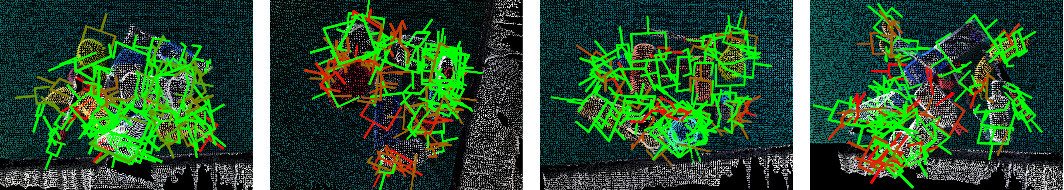
\includegraphics[width=0.98\linewidth]{figs/vg_result}
  \caption{Baseline}  
  \end{subfigure}  
  \begin{subfigure}[b]{0.98\linewidth}
    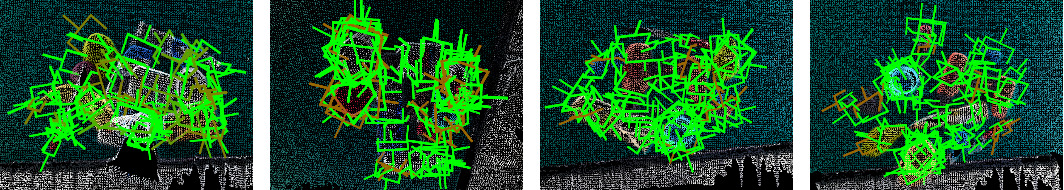
\includegraphics[width=0.98\linewidth]{figs/nvg_result}
  \caption{Ours}  
  \end{subfigure}  
    
  \caption{Examples of input scenes and predicted grasps from VoteGrasp \cite{hoang2022context} and the proposed method. The different intensity of grasp color denotes the confidence score of grasps. Green refers to the highest quality grasps and red refers to the lowest ones.}
  \label{fig:grasp_result}
\end{figure*}
%%%%%%%%%%%%%%%%%%%%%%%%%%%%%%%%%%%%%%%%%%%%%%%%%%%%%%%%%%%%%%%%%%%%

\subsection{Implementation Details}
\label{sec:implement}

%%%%%%%%%%%%%%%%%%%%%%%%%%%%%%%%%%%%%%%%%%%%%%%%%%%%%%%%%%%

\begin{table}[h]
\caption{Layer parameters of PointNet++ \cite{qi2017pointnet++} based feature learning network.}
\label{tab:layer_specs}
\begin{center}
\begin{tabular}{|l|c|c|}
\hline
layer name & input layer & layer params \\
\hline
SA1 & point cloud & (2048,0.025,[64,64,128]) \\
SA2 & SA1  & (1024,0.05,[128,128,256]) \\
SA3 & SA2 & (512,0.1,[128,128,256]) \\
SA4 & SA3 & (256,0.2,[128,128,256]) \\
FP1 & SA3, SA4 & [256,256] \\ 
FP2 & SA2, SA3 & [256,256] \\
\hline
\end{tabular}
\end{center}
\end{table}
%%%%%%%%%%%%%%%%%%%%%%%%%%%%%%%%%%%%%%%%%%%%%%%%%%%%%%%%%%%

In our implementation\footnote{Our code and other materials are available at \url{https://github.com/hoangcuongbk80/NovelVoteGrasp}}, we employ a pre-trained ResNet34 model trained on the ImageNet dataset as the encoder for RGB images. The output appearance feature from this encoder-decoder architecture comprises 256 channels. For point cloud feature extraction, we randomly sample 12,288 points from depth images and utilize a PointNet++ \cite{qi2017pointnet++}-based feature learning network, which also yields a 256-channel output. The detailed layer parameters of PointNet++ \cite{qi2017pointnet++} are displayed in Table~\ref{tab:layer_specs}. In the voting and context learning modules, we form $K=128$ clusters and produce a new feature map $\mathcal{F}_{context} \in 128 \times 512$. Subsequently, 128 grasps are generated from this new feature map. The prediction layer comprises $5 + V + 2A$ channels, with $V=120$ and $A=6$. We set $\lambda_{1}=\lambda_{2}=1.0$ and $\alpha$=$\beta$=$\gamma$=1.0. Our network is trained entirely using a batch size of 8 and optimized with Adam, employing a learning rate of 0.001 for 200 epochs. Training on a single Nvidia GeForce RTX 2080 Ti 11GB GPU takes approximately 20 hours. Regarding inference, our method requires 90ms for a single scene during the forward pass.

\subsection{Evaluation on GraspNet-1Billion}

We follow previous research \cite{fang2020graspnet} and evaluate our results on the dataset using $Precision@k$. This metric quantifies the precision of the top-k ranked grasps. To identify a predicted grasp ($G_{p}$) as a true positive, it must satisfy three conditions: (i) containing an object inside the gripper; (ii) being collision-free; (iii) exhibiting an antipodal grasp under a given friction coefficient $\mu$. The third condition is calculated based on prior works \cite{ten2017grasp, fang2020graspnet}. We denote $AP_{\mu}$ as the average $Precision@k$ for $k$ values ranging from 1 to 50, given a friction coefficient $\mu$. Additionally, we present the average of $AP_{\mu}$ across $\mu = \left\lbrace 0.2,0.4,0.6,0.8,1.0 \right\rbrace $, denoted as $AP$.


\begin{table*}[h]
\caption{The table shows the results on GraspNet-1Billion test set captured by RealSense/Kinect sensors respectively.}
\label{tab:grasp_detect_eval}
\begin{center}
\begin{tabular}{|l|c|c|c|c|c|c|c|c|c|}
\hline
& \multicolumn{3}{c|}{Seen} & \multicolumn{3}{c|}{Unseen (but similar)} & \multicolumn{3}{c|}{Novel} \\
\hline
& $AP$ & $AP_{0.8}$ & $AP_{0.4}$ & $AP$ & $AP_{0.8}$ & $AP_{0.4}$ & $AP$ & $AP_{0.8}$ & $AP_{0.4}$  \\
\hline
GG-CNN \cite{morrison2018closing} & 15.5/16.9 & 21.8/22.5 & 10.3/11.2 & 13.3/15.1 & 18.4/19.8 & 4.6/6.2 & 5.5/7.4 & 5.9/8.8 & 1.9/1.3 \\
\hline
Chu et al. \cite{chu2018real} & 16.0/17.6 & 23.7/24.7 & 10.8/12.7 & 15.4/17.4 & 20.2/21.6 & 7.1/8.9 & 7.6/8.0 & 8.7/9.3 & 2.5/1.8 \\
\hline
GPD \cite{ten2017grasp} & 22.9/24.4 & 28.5/30.2 & 12.8/13.5 & 21.3/23.2 & 27.8/28.6 & 9.6/11.3 & 8.2/9.6 & 8.9/10.1 & 2.7/3.2 \\
\hline
PointNetGPD \cite{liang2019pointnetgpd} & 26.0/27.6 & 33.0/34.2 & 15.4/17.8 & 22.7/24.4 & 29.2/30.8 & 10.8/12.8 & 9.2/10.7 & 9.9/11.2 & 2.7/3.2 \\
\hline
Fang et al. \cite{fang2020graspnet} & 27.6/29.9 & 33.4/36.2 & 17.0/19.3 & 26.1/27.8 & 34.2/33.2 & 14.2/16.6 & 10.6/11.5 & 11.3/12.9 & 4.0/3.6 \\
\hline
Gou et al. \cite{gou2021rgb} & 28.0/32.1 & 33.5/39.5 & 17.8/20.9 & 27.2/30.4 & 36.3/37.9 & 15.6/18.7 & 12.3/13.1 & 12.5/13.8 & 5.6/6.0 \\
\hline
Contact-GraspNet \cite{sundermeyer2021contact} & 29.9/31.4 & 35.2/39.0 & 19.5/21.6 & 28.2/29.0 & 37.0/35.2 & 16.3/18.9 & 13.2/13.9 & 13.5/14.7 & 6.8/7.7 \\
\hline
VoteGrasp \cite{hoang2022context}  & 34.1/37.5 & 38.9/45.6 & 24.0/27.7 & 33.0/35.9 & 40.8/43.3 & 20.5/24.7 & 16.9/18.5 & 17.0/18.5 & 10.0/10.6 \\
\hline
Ours (-VGG)  & 32.0/35.1 & 36.4/43.7 & 22.1/25.4 & 31.0/33.8 & 38.3/41.2 & 18.3/22.4 & 14.8/16.1 & 15.0/16.3 & 9.1/9.3 \\
\hline
Ours (-GGV)  & 31.4/34.6 & 35.4/42.1 & 21.4/24.2 & 30.0/32.1 & 37.4/40.0 & 17.0/21.2 & 13.5/15.8 & 14.8/15.5 & 8.3/8.8 \\
\hline
Ours & \textbf{38.5}/\textbf{39.2} & \textbf{43.1}/\textbf{46.7} & \textbf{29.3}/\textbf{30.8} & \textbf{37.2}/\textbf{38.0} & \textbf{44.1}/\textbf{45.2} & \textbf{25.1}/\textbf{28.1} & \textbf{21.5}/\textbf{21.2} & \textbf{22.5}/\textbf{22.9} & \textbf{12.6}/\textbf{13.2} \\
\hline
\end{tabular}
\end{center}
\end{table*}
%%%%%%%%%%%%%%%%%%%%%%%%%%%%%%%%%%%%%%%%%%%%%%%%%%%%%%%%%%%%%%%%%%%%

Table \ref{tab:grasp_detect_eval} and Fig. \ref{fig:grasp_result} demonstrate the performance comparison between our approach and state-of-the-art methods. The evaluation utilized the evaluation metric adopted in \cite{fang2020graspnet}, enabling a direct comparison with related works reported in \cite{fang2020graspnet, gou2021rgb}. The table showcases the evaluation outcomes categorized into "Seen," "Unseen (but similar)," and "Novel" objects, aiding in assessing the model's generalization capability. The results indicate superior performance on scenes featuring seen objects across all methods, while notably, our proposed approach consistently outperforms others, even in the challenging "Novel" category, underscoring its robust generalization capabilities.

The distinctions between "Ours (-VGG)" and "Ours (-GGV)" when compared to our complete approach ("Ours") showcase the significant impact of these modules. When excluding the VGG module, the method lacks the ability to effectively integrate RGB features, leading to a considerable reduction in performance across all evaluation categories: Seen, Unseen (but similar), and Novel objects. Similarly, without the GGV module, the model fails to appropriately fuse depth-based features, resulting in notable performance degradation in grasp detection across the board. The performance drop in both cases reaffirms the critical role played by these modules in amalgamating complementary information from RGB and depth data. It highlights their significance in capturing nuanced visual cues from different sources, which are vital for accurate and robust grasp detection. This clear decline in performance underlines the necessity of the VGG and GGV modules in our model's architecture, demonstrating their collective contribution to a more comprehensive understanding of the scene by integrating information from diverse modalities. The substantial discrepancy in results showcases that these modules are not just supplementary but rather pivotal components in leveraging the combined strengths of RGB and depth information. Their absence leads to a significant loss in the model's ability to discern crucial features necessary for precise grasp detection, emphasizing the vital role of these fusion modules in enhancing the model's performance across various object scenarios.

\textbf{Computational Time.} Our experiments were conducted on an Intel Xeon E-2716G CPU clocked at 3.7 GHz, paired with an Nvidia GeForce RTX 2080 Ti GPU featuring 11GB of memory. The runtime analysis of all evaluated methods is graphically represented in Fig. \ref{fig:runtime}. Our approach achieves a runtime of 100 ms per RGBD image. This fine balance between accuracy and speed empowers our method to proficiently generate grasp configurations in cluttered scenes, rendering it well-suited for diverse real-world scenarios.

%%%%%%%%%%%%%%%%%%%%%%%%%%%%%%%%%%%%%%%%%%%%%%%%%%%%%%%%%%%%%%%%%%%%
\begin{figure}
\centering
	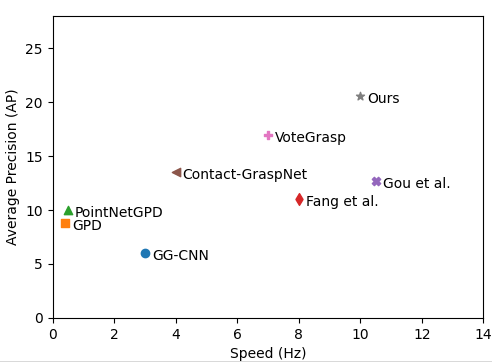
\includegraphics[width = 0.98\linewidth]{figs/time}
\caption{Comparison of running speed (Hz) and AP on GraspNet-1Billion
dataset.}
\label{fig:runtime}
\end{figure}
%%%%%%%%%%%%%%%%%%%%%%%%%%%%%%%%%%%%%%%%%%%%%%%%%%%%%%%%%%%%%%%%%%%%

\subsection{Robotic Grasping Experiment}
\label{sec:real_grasping}

The experiments were conducted with a Franka Emika Panda robot arm with 7-DOF, equipped with a parallel-jaw gripper as shown in Fig.~\ref{fig:robot1}. To capture RGBD data, we used either ASUS Xtion PRO LIVE sensor or  Microsoft Kinect sensor v2. The whole system is implemented using the ROS and MoveIt! frameworks. \\

%%%%%%%%%%%%%%%%%%%%%%%%%%%%%%%%%%%%%%%%%%%%%%%%%%%%%%%%%%%%%%%%%%%%
\begin{figure}[h!]
  \centering
 
  
  \begin{subfigure}[b]{0.98\linewidth}
    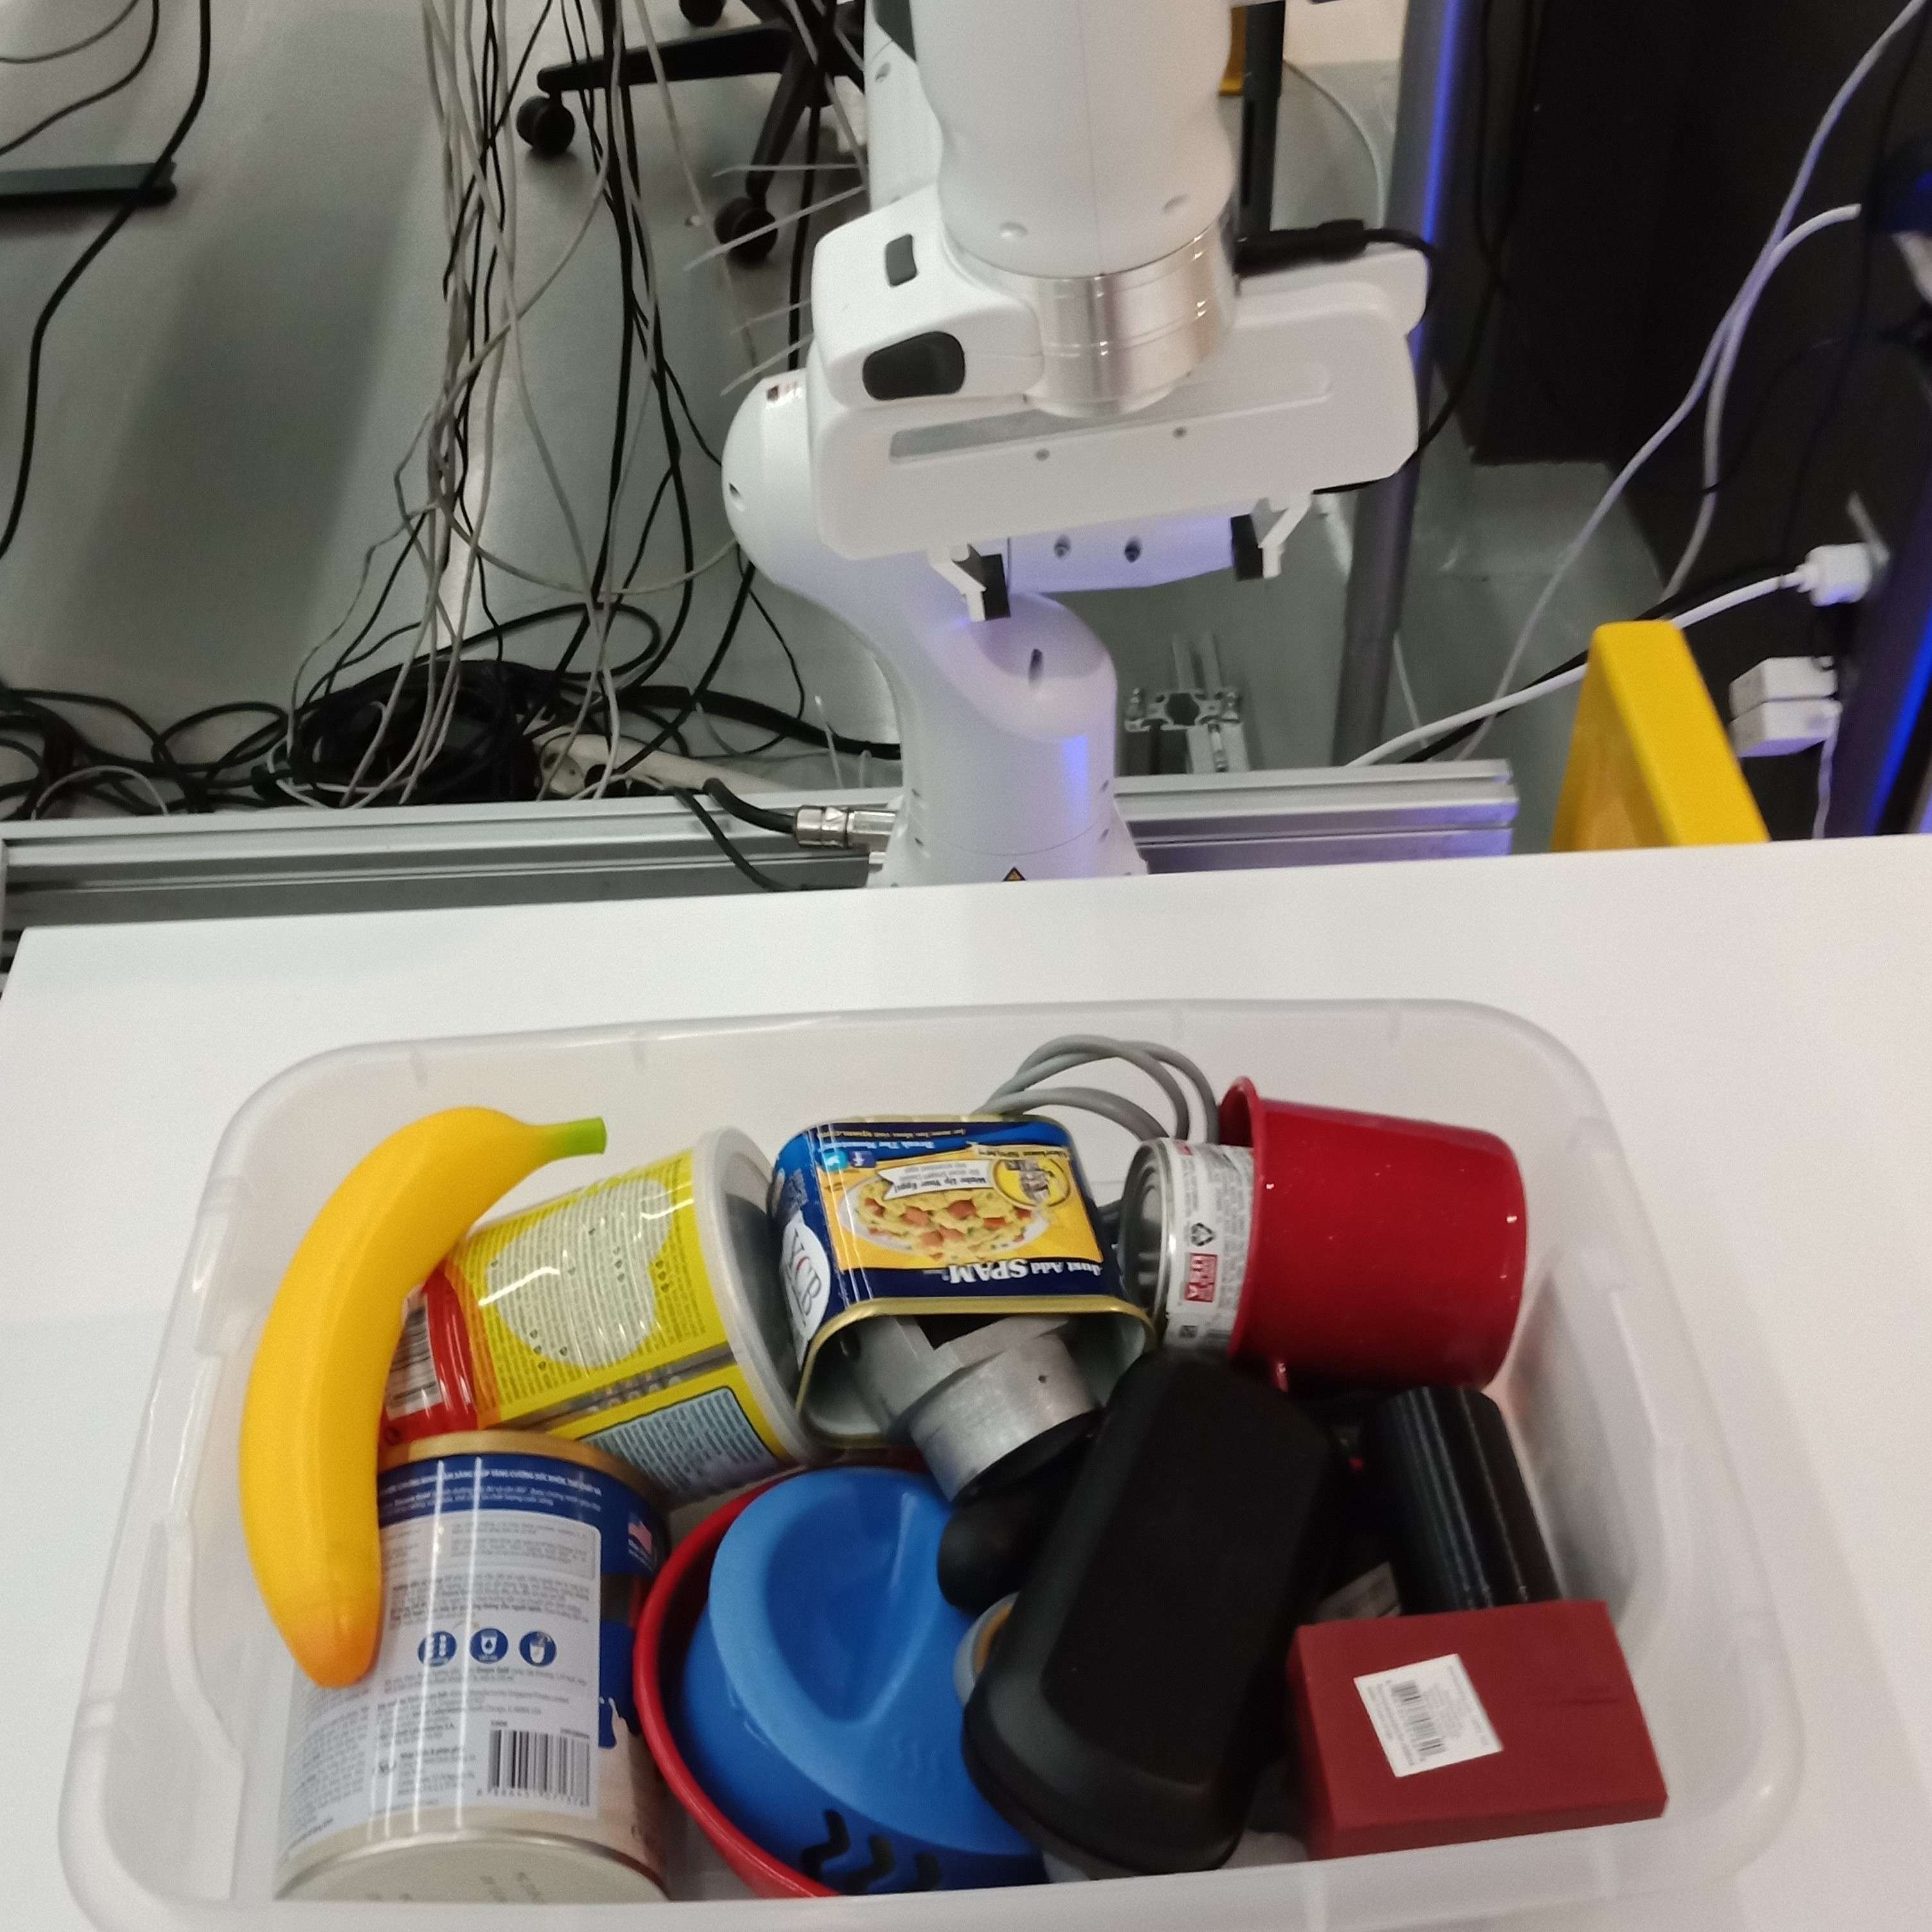
\includegraphics[width=0.48\linewidth]{figs/robot2}
    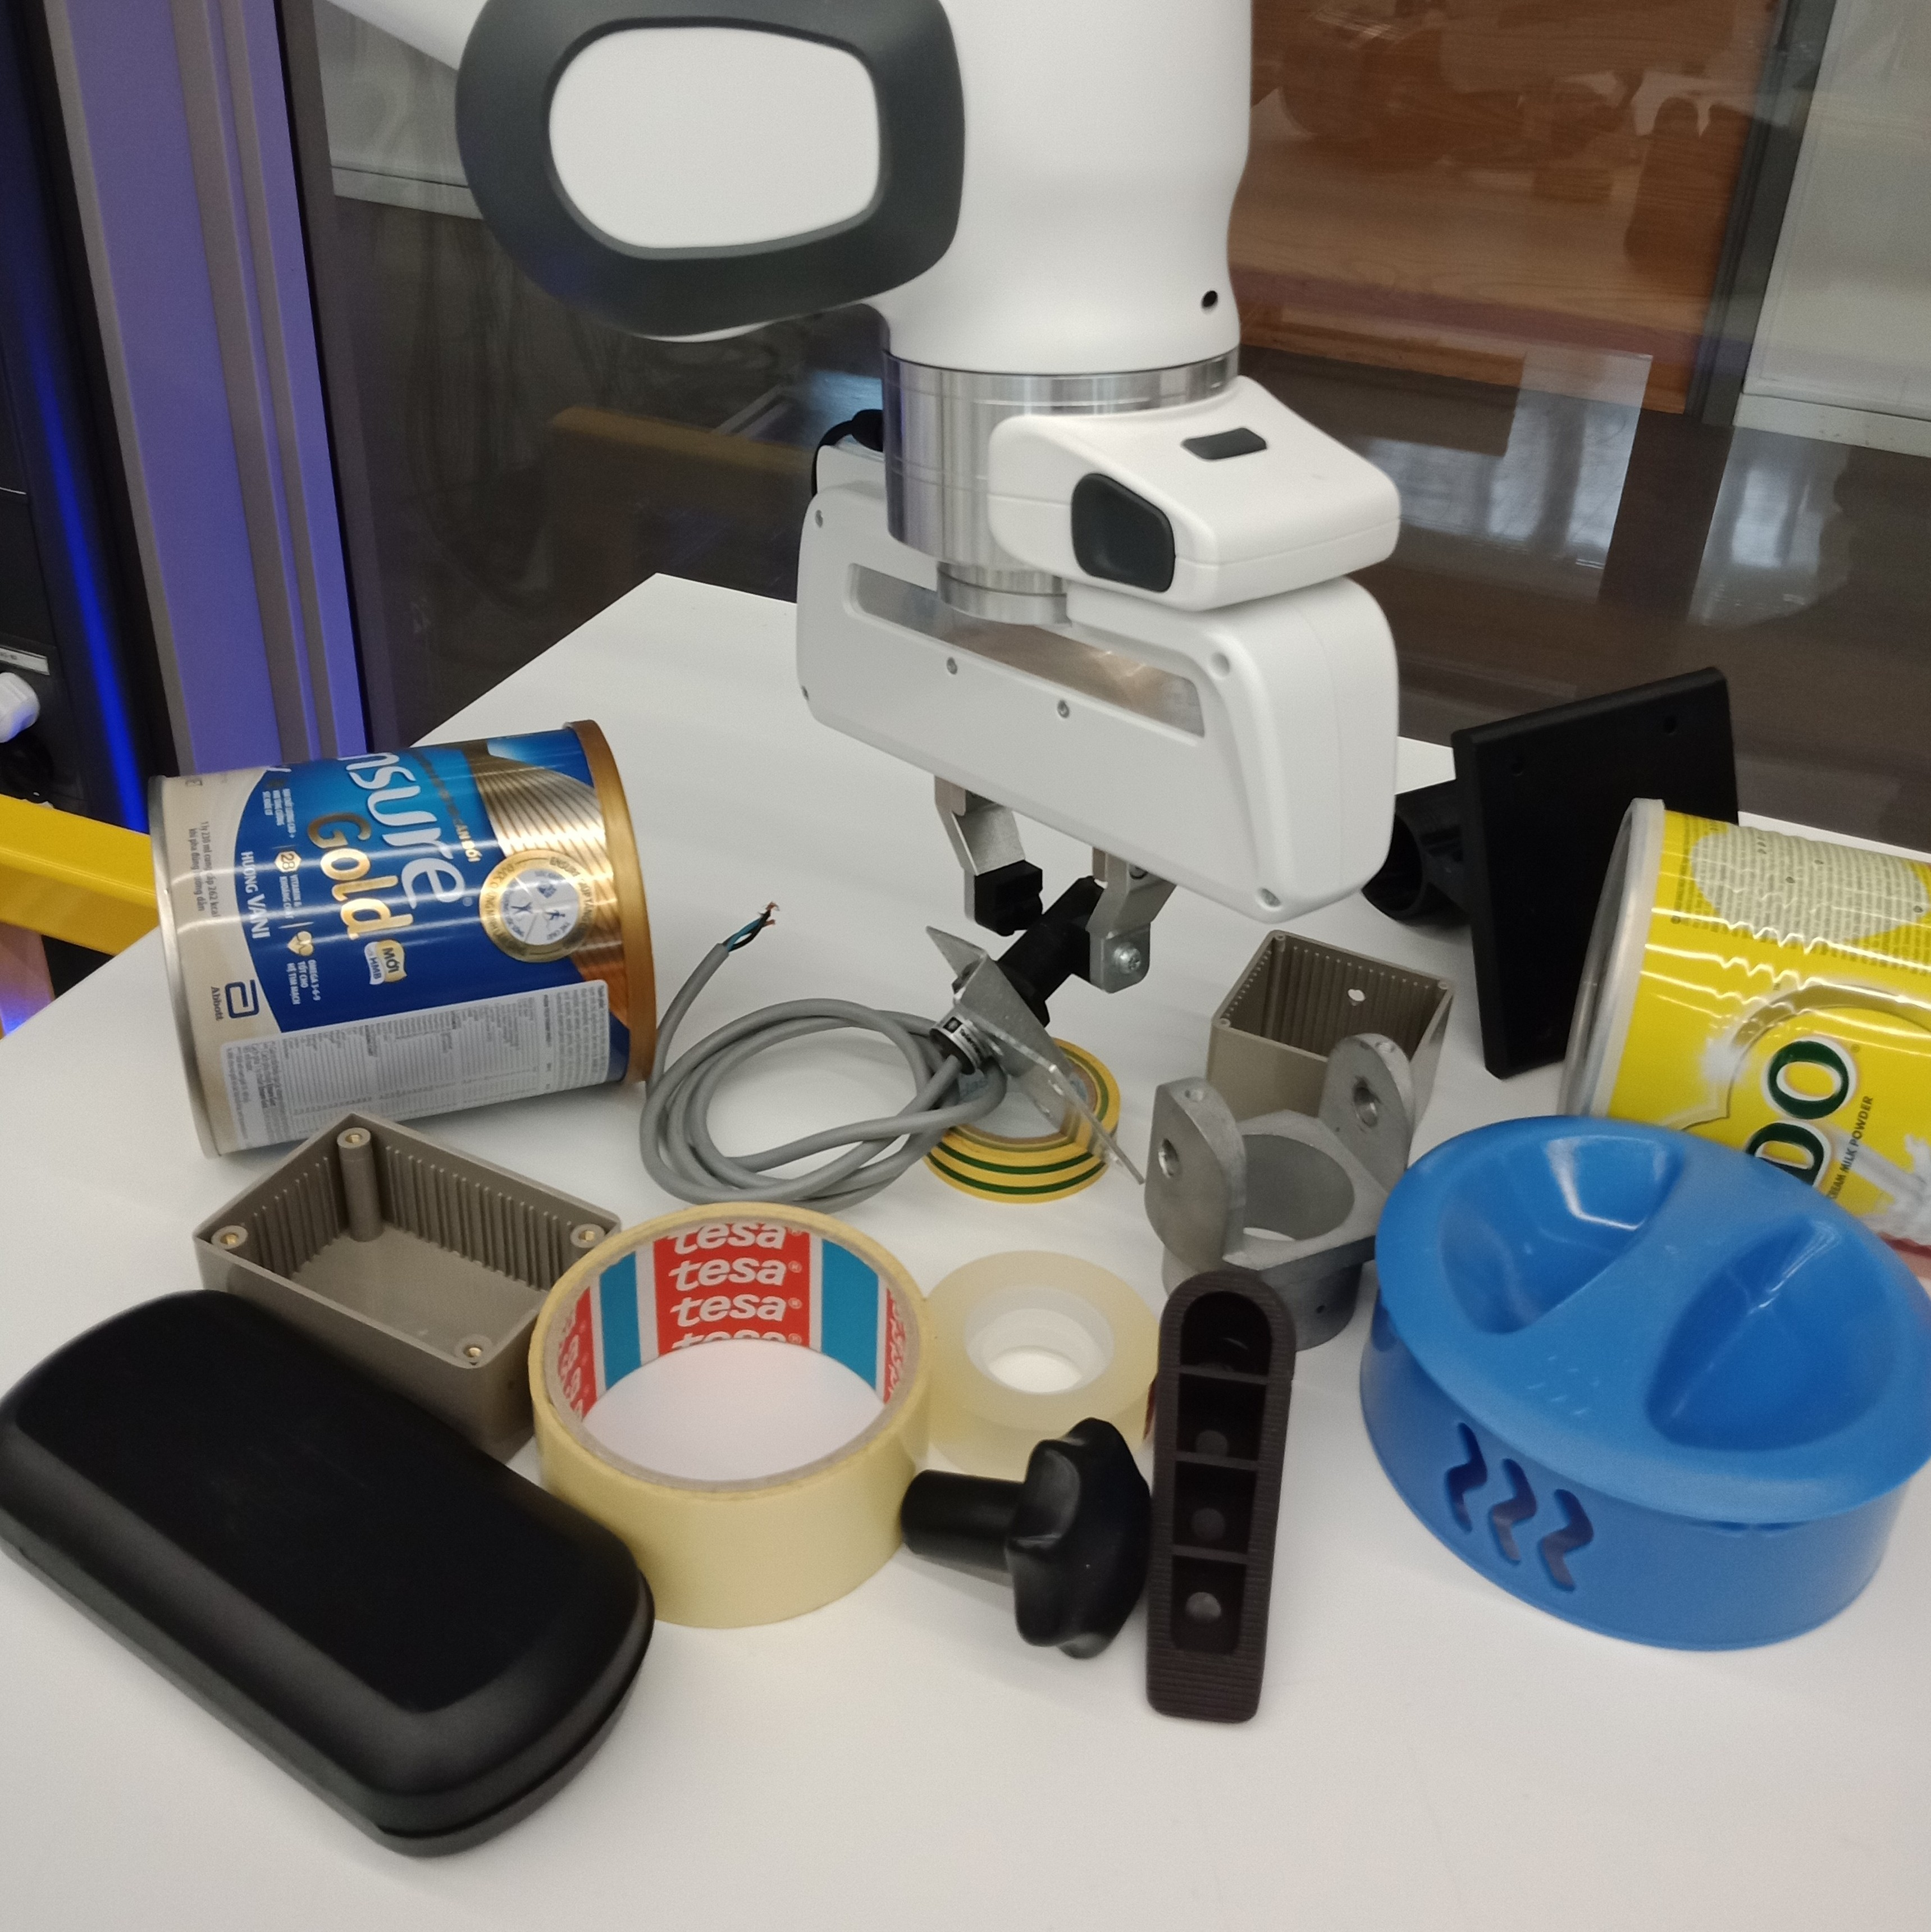
\includegraphics[width=0.48\linewidth]{figs/robot4} 
  \end{subfigure}
    
  \caption{Real-world grasping experiment.}
  \label{fig:robot1}
\end{figure}
%%%%%%%%%%%%%%%%%%%%%%%%%%%%%%%%%%%%%%%%%%%%%%%%%%%%%%%%%%%%%%%%%%%%

\begin{table}[h!]
\caption{Results of real robot experiments. The networks were trained on the GraspNet-1Billion dataset. The table shows the number of attempts, the number of successful attempts, and the grasp success rate.}
\label{tab:real_grasping}
\begin{center}
\begin{tabular}{|l|c|c|c|}
\hline
Method & Attempt & Success & Success Rate \\
\hline
GPD \cite{ten2017grasp} & 300 & 195 & 65\% \\
PointNetGPD \cite{liang2019pointnetgpd} & 300 & 201 & 67\% \\
Fang et al. \cite{fang2020graspnet} & 300 & 214 & 71\% \\
Gou et al. \cite{gou2021rgb} & 300 & 218 & 73\% \\
Contact-GraspNet \cite{sundermeyer2021contact}  & 300 & 222 & 74\% \\
VoteGrasp \cite{hoang2022context} & 300 & 234 & 78\% \\
Ours & 300 & \textbf{251} & \textbf{84}\% \\
\hline
\end{tabular}
\end{center}
\end{table}
%%%%%%%%%%%%%%%%%%%%%%%%%%%%%%%%%%%%%%%%%%%%%%%%%%%%%%%%%%%

We conducted a real-world evaluation of state-of-the-art grasp detection methods, each trained on the GraspNet-1Billion dataset for a fair comparison. GPD \cite{ten2017grasp}, PointNetGPD \cite{liang2019pointnetgpd}, and Contact-GraspNet \cite{sundermeyer2021contact} were trained using the hyperparameters specified in their respective papers. We selected novel objects tailored to fit the gripper's shapes and sizes. In each scenario, a random subset of 10-15 objects was arranged in a haphazard manner on a table, mirroring the unpredictability of real-world environments. Each method underwent 300 grasp attempts, with the robot randomly selecting objects. A grasp was deemed successful if the robot could grasp and lift the object within a single attempt. The results in Table \ref{tab:real_grasping} demonstrate our method's superiority, achieving an 84\% success rate outperforming all other methods. This highlights the proposed framework's efficacy in real-world grasping scenarios, attributing the increased success rate to the integration of estimated depth data, underscoring the significance of richer input data for precise and effective.  \\

\section{Conclusions}

In this study, we addressed the fundamental challenge of grasp generation in robotic manipulation by introducing an innovative approach that bypasses the need for specialized depth sensors. Our method revolutionizes grasp generation by leveraging tailored deep learning techniques to estimate depth from color (RGB) images directly. This paradigm shift allows the computation of predicted point clouds solely from RGB inputs, eliminating the dependency on traditional depth sensors. A pivotal contribution lies in the development of a fusion module adept at seamlessly integrating features derived from RGB images with those inferred from predicted point clouds. This fusion process harnesses the strengths of both modalities, significantly enhancing grasp configurations. Experimental evaluations unequivocally validate the effectiveness of our approach, demonstrating its superiority in generating grasp configurations compared to existing methods. Future endeavors in these outlined directions hold the promise of further enhancing the versatility, adaptability, and real-world applicability of grasp generation in robotics.
%

\bibliographystyle{ACM-Reference-Format}
\bibliography{References}

\end{document}
\endinput
%%
%% End of file `sample-sigplan.tex'.
